
%
% attack summary table in previous section for positioning
%

\section{Attacks}
\label{sec:attacks}
In this section, I demonstrate how an adversary can combine and
exploit the issues
% I have
described in Section~\ref{sec:assumptions} to create attacks that reliably
bypass existing anti-spoofing protections.  In particular, I consider an
attack successful if a spoofed email message is delivered to a
victim's inbox (\ie,  not the spam folder), and yet does not produce a
warning to the user.
Figure~\ref{fig:open_forwarding_attack_screenshot} shows
an example of a successful attack, where a spoofed
email purporting to be from \dns{bush@state.gov} is delivered to a
Gmail user's inbox with no warning indication.

I describe four distinct classes of attacks, summarized in
Table~\ref{tab:summary_attacks}, each of which I have validated
empirically using accounts created at the affected providers.  Some of
these attacks are quite broad --- allowing an attacker to spoof email
to any email recipient purporting to be from tens of thousands of
popular and sensitive domains --- while others are more circumscribed
in their impact.
%
For each of the attacks described below, I refer to the domain an
attacker specifies in their \textsc{FROM} header as the
\textit{spoofed domain}.  I use the terms \textit{spoofed address} to
refer to the full email address appearing in the \textsc{FROM} header
and \textit{forwarding domain} to refer to the domain of the
forwarder.

\begin{figure}[t]
  \centering
%% \centerline{\includegraphics[width=\columnwidth]{graphs/ss_outlook_open_forwarding.png}}
{
    \setlength{\fboxsep}{0pt}
    \setlength{\fboxrule}{0.5pt}
    \fbox{\includegraphics[trim=2 2 2 47,clip,width=0.7\columnwidth]{fig/ss_outlook_open_forwarding.png}}
}
%  \vspace*{-0.2in}
  \caption[Example of a Successful Attack]{Example of a successful attack. A spoofed email purporting to be \dns{bush@state.gov} is delivered to a Gmail user's inbox with no warning indicators.
}
%\vspace*{-0.1in}
\label{fig:open_forwarding_attack_screenshot}
\end{figure}


\begin{figure*}[t]
  \centerline{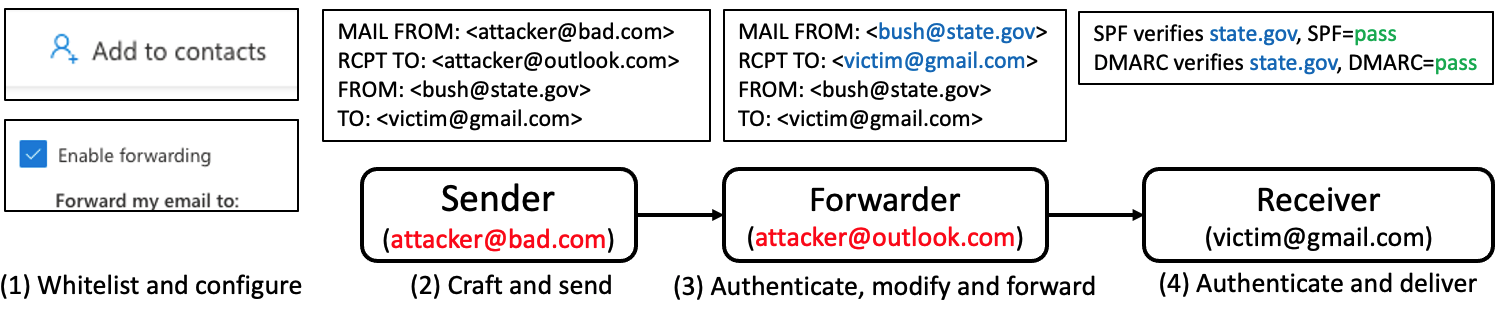
\includegraphics[width=\textwidth]{fig/mech_outlook_open_forwarding.pdf}}
  \centering
  \caption[Example of an SPF Incorporation Attack]{Example of an SPF Incorporation Attack (\S~\ref{subsec:attack_open_forwarding}) exploiting Outlook's open forwarding to spoof email from domains incorporating Outlook's SPF records (e.g., \dns{state.gov}) to arbitrary recipients.}
  \label{fig:open_forwarding_attack_mechanism}
  %    \vspace*{-0.1in}
\end{figure*}


\paragraph{Threat Models}
For the first three attacks, I assume an adversary controls the
sender and forwarding accounts: they possess a server capable of
sending spoofed email messages (sender) and a personal account with a
specific third-party provider that allows \emph{open forwarding}
(forwarder). For the attack described in
Section~\ref{subsec:attack_none_mailing_list}, I make three
assumptions: (a) that adversaries control a malicious server that can
send spoofed email messages and try to spoof email from a domain that
hosts a mailing list with REM forwarding (e.g., Google Groups,
Listserv and Mailman as described in
Section~\ref{sec:measure_forwarding_mechs_and_arc}), (b) that the spoofed domain
has a DMARC policy of \textsc{None} (all too common); and (c) the
sending email address the attacker wishes to impersonate has
permission to send to the mailing list.

%We validated each of these attacks empirically using
%accounts I created with each of the affected providers.
%Additionally, I have disclosed all of these vulnerabilities to the
%affected providers (Section~\ref{sec:disclosure}).

%We also demonstrate how an adversary can ``launder'' spoofed email
%through mailing lists, such that the resulting spoofed email also
%passes SPF and DMARC validation checks.


%% include email addressed from: (1) any
%% domain that incorporates Outlook's SPF information in their SPF
%% records (\ie, including thousands of high-profile domains such as
%% \dns{state.gov}, \dns{disneyplus.com}, and \dns{qantas.com}),\alex{do I still want to say any domain} (2) any
%% domain, if the recipient is a Zoho user, and (3) any domain with a
%% DMARC policy of none or quarantine (\eg, \dns{alipay.com}), if the
%% recipient is a Gmail user.

%\grant{I'm not sure how I feel about the caveats about specific email provider. They seem to detract / complicate the impact examples and I wonder if others feel the same or see a way to word them more broadly (e.g., in terms of forwarding approaches, rather than specific providers).}
%\geoff{since I have even more qualifiers on the attacks than before (e.g., Alex's note about any domain no longer being accurate), how about if I reduce this part to something on the order of ``in some cases impacting ....''}

% For the remainder of this section, we
% describe each of these attacks in detail and explain what enables each
% to bypass existing anti-spoofing measures.

%Each attack combines vulnerable forwarding features (\S~\ref{subsec:fwding_vuln}) and/or the header rewriting performed by common forwarding approaches (\S~\ref{sec:background:fwdingflow}) to violate security assumptions made by anti-spoofing defenses (\S~\ref{subsec:assumptions}).
%While these defenses would have mitigated spoofing in a direct email transmission settings, the use of forwarding enables successful spoofing attacks.
% For each attack, I describe the steps an attacker performs to successfully spoof an email and explain how forwarding,
% combined with the vulnerabilities from Section~\ref{sec:assumptions} enable the attack to bypass anti-spoofing measures.
 % and will report on their feedback in a final version of this paper.

% In all four attacks, I assume that the adversary controls their own SMTP server for sending spoofed email messages (i.e., the sender is malicious). Additionally, for the first three attacks, I assume that the adversary also controls personal email accounts registered with the forwarder, which is easily done with services like Outlook and Fastmail. For the last attack involving mailing lists, I assume that the adversary knows a target email address within the organization that is allowed to send to the mailing list.


\begin{figure*}[t]
  \centerline{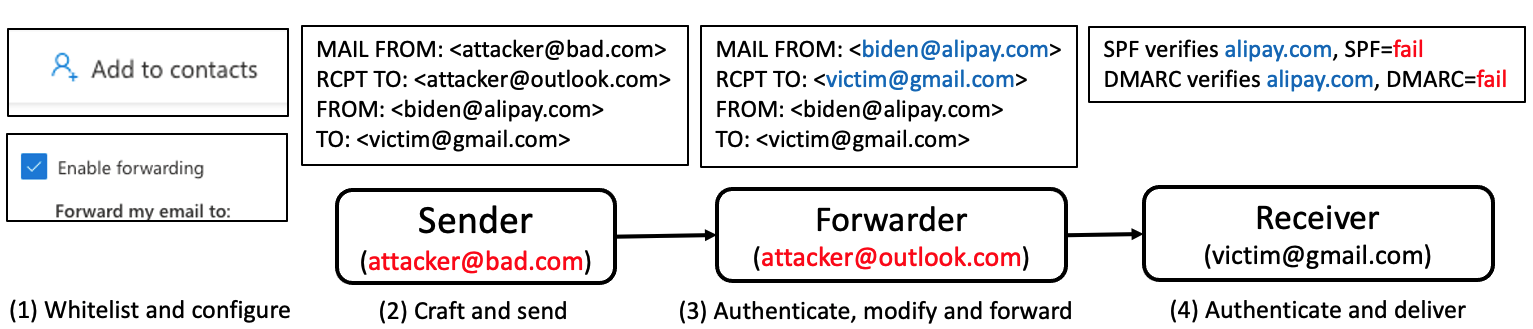
\includegraphics[width=\textwidth]{fig/mech_gmail_via_outlook.pdf}}
  \centering
  \caption[Example of a Spoofed Email Attack Exploiting Open Forwarding]{Example of a spoofed email attack exploiting open forwarding and relaxed validation for forwarded email from well-known providers (\S~\ref{subsec:attack_relaxed_forwarding_validation}).
    Note that the spoofed domain, \dns{alipay.com}, has a DMARC policy of Quarantine and thus
    % its traffic
    should not be delivered.}
  \label{fig:mech_gmail_via_outlook}
\end{figure*}


\subsection{Exploiting SPF Incorporation}
\label{subsec:attack_open_forwarding}

% \subsubsection*{Attack Overview}
The first attack I describe exploits five discrete issues:
three security assumptions (\S~\ref{subsubsec:spf_incorporation},~\ref{subsubsec:quarantine_instead_of_reject},~\ref{subsubsec:whitelist}),
the vulnerable \emph{open forwarding} feature that many providers offer (\S~\ref{subsubsec:open_forwarding}),
and the header rewriting performed as part of the PMF and MFEF forwarding approaches (\S~\ref{sec:measure_forwarding_mechs_and_arc}).
Crucially,
%as described in Section~\ref{subsubsec:spf_incorporation},
the rise of large third-party email providers violates SPF's assumption that the set of authorized server IP addresses specified by each domain cannot be used by other domains or external users to send email.
% SPF assumes that set of authentic server IP addresses that each domain specifies cannot be used by other domains or external users to send emails. The rise of third-party providers has challenged this assumption --- many domains now outsource their email services to these third-party email providers.
For example, the owners of domain \dns{state.gov} use Outlook as their email provider.  Thus, email messages sent by \dns{state.gov}'s employees will originate from Outlook's mail servers.
To ensure reliable delivery, such domains routinely add the server IP addresses of their email provider to their own SPF records.
Although intuitive, this configuration creates an overly broad trust assumption: by adding the provider IP addresses to their SPF record, such domains (e.g., \dns{state.gov}) implicitly grant permission for any account hosted by their provider, whether individual or corporate, to send email messages that purportedly come from their domain.
This threat is only prevented because large providers like Outlook do not allow users to arbitrarily set or forge their email's FROM header.

However, I observe that by combining header rewriting from PMF and MFEF and the use of \emph{open forwarding}, attackers can overcome this defense and exploit SPF's violated assumption.
Specifically, this attack allows an adversary to spoof email from domains that incorporate a third-party provider's SPF information in their own SPF record to any recipient, regardless of the domain's DMARC policy.
%absent additional protections.

% Outlook also enables \emph{open forwarding} and uses the MFEF forwarding approach, which provides attackers with a mechanism for sending email messages with forged FROM headers.
% While Microsoft does not provide a mechanism for forging the FROM header, a malicious sender can spoof as arbitrary domain in the FROM header. With open forwarding, an adversary can create an individual Outlook account and use it to redirect an email with a forged FROM header to an arbitrary destination without verification.
% Together, these issues allow an adversary to reliably spoof as any domain that incorporates a third-party provider's SPF information in their own SPF absent some other protection.
% \subsubsection*{Impact}
%\paragraph{Impact}
\paragraph{Scope}
This attack works for domains that include the SPF record of any of six
large email providers (Outlook, iCloud, Freemail, Hushmail, Mail2World and Runbox) in their own SPF records.  Notably, given
Outlook's importance as a third-party provider~\cite{liu2021s}, this
attack allows an attacker to spoof email on behalf of tens of
thousands of popular domains.

Indeed, over 12\% of the Alexa 100K
most popular domains are vulnerable as a result (and almost 8\% of the
top 1M domains).  A cursory examination of this list identified a
range of potentially sensitive domains such as those hosting large
news reporting organizations (\eg, \dns{washingtonpost.com},
%\dns{cbsnews.com},
\dns{latimes.com},
%\dns{slate.com}, \dns{npr.org},
and \dns{apnews.com}),
%\dns{nydailynews.com} and \dns{afp.com}),
financial services (\eg,
%\dns{usbank.com}, \dns{discover.com},
\dns{mastercard.com}, \dns{transunion.com},
%\dns{fidelity.com},
and \dns{docusign.com}),
domain registrars (\eg, \dns{godaddy.com}),
certificate authorities (\eg,
\dns{sectigo.com} and \dns{digicert.com}) and large law firms (\eg,
\dns{perkinscoie.com}).  In addition, 32\% of US \dns{.gov} domains are
vulnerable (including 22\% of the domains used by Federal
agencies).  At the Federal level this includes the majority of US
cabinet organizations (\eg, \dns{state.gov}, \dns{dhs.gov} and
\dns{doe.gov}), a range of security sensitive agencies (\eg,
\dns{odni.gov}, \dns{cisa.gov} and \dns{secretservice.gov}) as well
as those charged with public health and safety (such as
\dns{fema.gov}, \dns{nih.gov}, and \dns{cdc.gov}).
%% \footnote{To say
%%   nothing of other critical government functions such as the funding
%%   of scientific research (\eg  nsf.gov).}
At the state and local
level, virtually all primary state government domains (\eg, \dns{mass.gov})
  are vulnerable (including a broad range of congress, judiciary,
  and law enforcement domains in each state) and over 40\% of all \dns{.gov}
  domains used by cities.\footnote{We have not broadly examined domains representing government offices outside the US, but I note that both \dnsfn{gchq.gov.uk} and \dnsfn{ncsc.gov.uk} are also vulnerable.}


% \footnote{Our estimation suggests that roughly
% 12.4\% of Alexa top $100K$ domains and 38.1\% of \dns{.gov} domains are
% vulnerable to this attack absent some other protection
% mechanism.
% This list includes both popular commercial domains such as \dns{disneyplus.com},  \dns{hulu.com} and \dns{qantas.com} and sensitive domains used by the U.S. government in its official capacity such as \dns{state.gov}, \dns{nsf.gov}, \dns{cdc.gov} and \dns{cisa.gov} among many others.}.


%% %Absent additional per-domain protections by
%% %Outlook(\S~\ref{subsubsec:whitelist}), this attack can be used to spoof any domain that incorporates Outlook's SPF information in their SPF
%% %record, regardless of the domain's DMARC settings (e.g., even with a
%% %policy of Reject).  Additionally, they can successfully deliver this
%% %spoofed email to any recipient at any email provider.
%% %\geoff{revisit: qualify this slightly in light of aa.com}
%% %
%% Figure~\ref{fig:open_forwarding_attack_mechanism} shows an example of
%% this attack using Outlook as the forwarding service. It consists of four stages.
%% %\label{subsubsec:open_forwarding_attack_mechanism}
%% %\alex{Updated the text}\grant{Would it work to incorporate this email forging as part of Stage 1,
%% %perhaps even just as text (Without changing the diagram).
%% %It's a little weird that I list some actions the attacker needs to do, and then talk about ``Stage 1'' and what the attacker does.}
%% An attacker starts by creating a personal account for
%% forwarding (\dns{attacker@outlook.com}), adding the spoofed address
%% (\dns{bush@state.gov}) to the account's ``allowlist'' (thereby
%% preventing any quarantining by Outlook), and configuring the account to
%% forward all email to the desired target (\dns{victim@gmail.com}). In this case, the spoofed domain \dns{state.gov} includes
%% Outlook's SPF record (\dns{spf.protection.outlook.com}) into its own SPF record and has a DMARC policy of \textsc{Reject}. Next, the attacker forges an email that purportedly originates from \dns{state.gov} and sends it to their personal Outlook account. Then, even though the message fails DMARC validation, Outlook will still forward it because the spoofed address is present in the account's allowlist.

  
  
% \subsubsection*{Threat Model and Attack Procedure}
%\paragraph{Attack Procedure}
\paragraph{Example}
%% \alex{another version of the above paragraph that works in the assumptions.}
% (need to reference the figure somewhere)
Figure~\ref{fig:open_forwarding_attack_mechanism} shows an example of
this attack using Outlook as the forwarding service.
An attacker starts by creating a personal account for
forwarding (\dns{attacker@outlook.com}), adding the spoofed address
(\dns{bush@state.gov}) to the account's ``allowlist'' (thereby
preventing any quarantining by Outlook), and configuring the account to
forward all email to the desired target (\dns{victim@gmail.com}). In this case, the spoofed domain \dns{state.gov} includes
Outlook's SPF record (\dns{spf.protection.outlook.com}) into its own SPF record and has a DMARC policy of \textsc{Reject}. Next, the attacker forges an email that purportedly originates from \dns{state.gov} and sends it to their personal Outlook account. Normally, Outlook would quarantine this email because it fails DMARC validation (\S~\ref{subsubsec:quarantine_instead_of_reject}). However, since the spoofed address is present in the account's allowlist, this configuration overwrites the quarantine decision (\S~\ref{subsubsec:whitelist}), and as a result, Outlook would forward the spoofed email to the target.


As per Outlook's MFEF forwarding implementation,
%the
\textsc{MAIL FROM}
%header
is rewritten to match the
\textsc{FROM} header, \dns{bush@state.gov} in our example. Finally, the recipient's mail server receives the forwarded email
and performs authentication checks.
From the recipient's perspective,
the spoofed email passes SPF validation because the
\textsc{MAIL FROM} domain (\dns{state.gov}) lists Outlook's SPF
information in its SPF record, and the forwarding configuration
arranged by the attacker ensures that the recipient receives this
spoofed email from Outlook's servers.
Moreover, this attack also
ensures that DMARC's alignment check succeeds because the
\textsc{MAIL FROM} and \textsc{FROM} domain are both \dns{state.gov}.
%\stefan{I don't think I need the screenshot.  I think they will believe us}
%\alex{nope I need this one}
I validated this attack in practice, consistently sending
spoofed email messages such as the example
shown in Figure~\ref{fig:open_forwarding_attack_screenshot}
to our own Gmail account, where it was delivered to the inbox without warning.\footnote{
Note that I did discover some exceptions in our experiments.
For a small set of high-profile domains that have a DMARC policy of Reject
(\eg, \dnsfn{aa.com}, \dnsfn{foxnews.com} and \dnsfn{ikea.com}), Outlook would
quarantine spoofed email regardless of whether users have added the
spoofed address to their account's allowlist (Section~\ref{subsubsec:quarantine_instead_of_reject}).
I surmise that Outlook applies special protections for a set of high-profile or frequently spoofed domains.
} 
In addition to Outlook, this attack also succeeds with
% five other large email providers:
iCloud, Freemail, Hushmail, Mail2World and Runbox.


\subsection{Abusing Relaxed Forwarding Validation}
\label{subsec:attack_relaxed_forwarding_validation}

% \subsubsection*{Attack Overview}
The second attack exploits the fact that many email providers apply relaxed validation policies to forwarded mail (\S~\ref{subsubsec:relaxed_validation}), particularly when messages arrive from well-known mail providers.
When combined with open forwarding, an attacker can abuse this behavior
to spoof email from any domain that has a DMARC policy of
%\geoff{is an and valid here?}\alex{yes. for gmail it is None and Quarantine}
\textsc{Quarantine} (or \textsc{None}) to any mail server that applies these relaxed measures (\eg, Gmail and Outlook).  Recall that, in the absence of forwarding, attackers cannot spoof email from a domain with a DMARC policy of \textsc{Quarantine}.
Provider-specific defenses, such as when Outlook quarantines any email that fails DMARC (\S~\ref{subsubsec:dmarc_none}), will also stop such direct, single-hop attacks.

\begin{figure*}[t]
\centerline{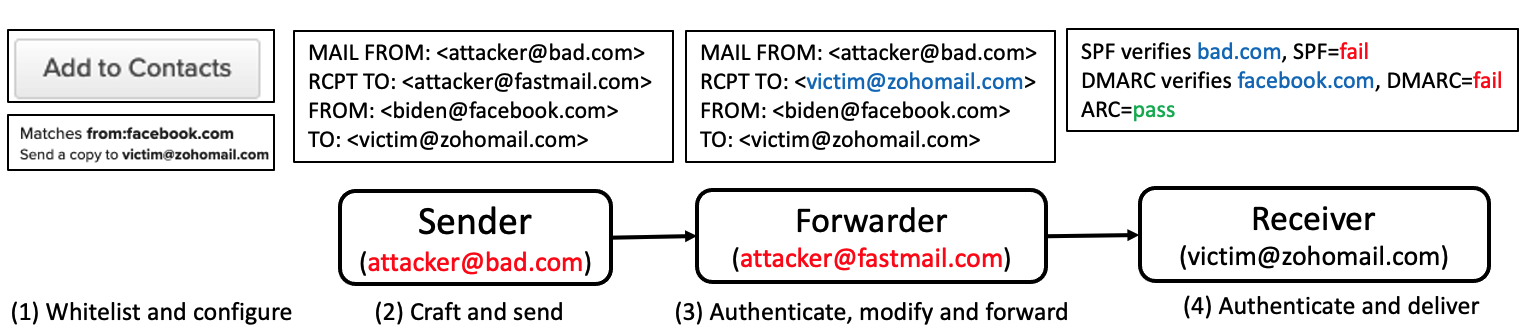
\includegraphics[width=\textwidth]{fig/mech_zoho_arc.pdf}}
\centering
\caption[Example Attack Exploiting Zoho's Vulnerable ARC Implementation]{Example attack that exploits Zoho's
vulnerable ARC implementation and  open forwarding to
  spoof email from arbitrary domains to any Zoho recipient (\S~\ref{subsec:attack_zoho_arc}).}
\label{fig:mech_zoho_arc}
%\vspace*{-0.1in}
\end{figure*}

% \subsubsection*{Impact}
%\paragraph{Impact}
\paragraph{Scope}
As described earlier in Section~\ref{subsubsec:relaxed_validation}, Gmail and Outlook use relaxed validation checks for forwarded email.
I find that an adversary can mount this attack against users with
Gmail/Outlook email accounts as well as users who use GSuite and Outlook 365 for email services.\footnote{Mail.ru also uses relaxed validation, but since it is only applied to email forwarded via Gmail, which does not allow open forwarding, this attack does not work for Mail.ru.}
%As a result, this attack impacts
% who together have
% roughly 1.9 billion users worldwide~\cite{GmailWik42:online, Outlookc33:online}
% when taking into account both users with
% Gmail/Outlook email accounts, as well as all users who use GSuite and
% Outlook 365 for email services (who are also vulnerable)

% \subsubsection*{Threat Model and Attack Procedure}
%\paragraph{Attack Procedure}
\paragraph{Example}
Figure~\ref{fig:mech_gmail_via_outlook} illustrates the steps of this
attack using an example where the adversary creates a personal Outlook
account to forward spoofed email messages to Gmail recipients.  First,
the adversary selects a spoofed email address from a domain with a
DMARC policy of \textsc{Quarantine} or \textsc{None} (we use \dns{alipay.com} in this example, a prominent Chinese payment company), adds the address
to their forwarding account's allowlist, and configures their
forwarding account to send email to the victim (recipient).  Like the
first attack, the attacker then sends a message from this spoofed address
to their forwarding account, which is then forwarded to the recipient.

When the final recipient's mail server receives
the email, the server will observe that the email comes from a
``well-known'' provider, apply its relaxed validation checks, and
successfully deliver the email to the recipient's inbox (even though
the spoofed email fails normal SPF and DMARC checks).
%\alex{The part that talks about the UI bug}
%We verified this attack, and Figure~\ref{fig:ss_gmail_via_outlook} in the Appendix shows one such spoofed message delivered to GMail without security warnings.


\subsection{Targeting ARC Vulnerabilities}
\label{subsec:attack_zoho_arc}
% \subsubsection*{Attack Overview}
The third attack allows an adversary to deliver spoofed email messages
from arbitrary domains to Zoho users.  This attack exploits Zoho's
vulnerable implementation of the experimental Authenticated Received
Chain (ARC) protocol~\cite{ARCSpeci1:online}, which was first
documented by Shen et al.~\cite{shen2020weak}. Due to this bug, Zoho
incorrectly reads ARC headers and will deliver arbitrary email
messages with ARC headers added by providers such as Gmail and
Fastmail to the recipient's inbox without any warning.  However, I
show that this issue is not limited to interactions between Gmail and
Zoho customers.  I demonstrate how further issues, including the fact that
Zoho trusts and (incorrectly) reads ARC headers added by Fastmail, open forwarding
(\S~\ref{subsubsec:open_forwarding}), and several forwarding
assumptions (\S~\ref{subsubsec:quarantine_instead_of_reject},
\S~\ref{subsubsec:whitelist}), can be combined with the underlying ARC
vulnerability to allow an adversary to deliver spoofed email messages
from arbitrary domains to arbitrary Zoho users.

This attack again highlights the fact that email security protocols
are distributed and independently-configured components, where
vulnerable decisions by one party incur harm to downstream recipients
but not necessarily to their own users.  Notably, the actions taken
by one provider (e.g., Fastmail) can unexpectedly undermine the
security of users on another platform (e.g., Zoho).

%This attack works by combining several vulnerabilities: Zoho's vulnerable ARC implementation (more details below), 

%One main vulnerability exploited in this attack is Zoho's vulnerable
%implementation of the experimental Authenticated Received Chain (ARC)
%protocol~\cite{ARCSpeci1:online}, which was first documented by Shen
%et al.~\cite{shen2020weak}. Due to this bug, Zoho incorrectly reads
%ARC headers and will deliver arbitrary email messages with ARC headers
%added by providers such as Gmail and Fastmail to the recipient's inbox
%without any warning.

%To make this attack work, an adversary needs to
%exploit multiple different vulnerable forwarding assumptions and
%features, in addition to the flaw in Zoho's ARC implementation.
%We note that our work has not only led
%to a patch resolving this issue after disclosure to Zoho, but also
%resulted in Zoho adding additional security enhancements to their ARC
%implementation (Section~\ref{sec:disclosure}).
%\stefan{
%\grant{I'm commenting out the list of vulnerable things below because it seems redundant with both the intro paragraph and the attack description.}

% Importantly, several forwarding assumptions and open forwarding are required for this attack to work, in addition to Zoho's buggy ARC implementation. Namely, the attack I demonstrate in this section exploits that Fastmail allows open forwarding (Section~\ref{subsubsec:open_forwarding}), that Fastmail allow users to overwrite DMARC decisions through whitelisting (Section ~\ref{subsubsec:whitelist}), that Fastmail does not reject spoofed email messages addressed from domains with DMARC policy \textsc{REJECT} (Section~\ref{subsubsec:quarantine_instead_of_reject}), and that Zoho (incorrectly) reads ARC headers added by Fastmail (Appendix~\ref{sec:appendix_arc_measurement}). I provide more details in the example below.

%\paragraph{Impact}
\paragraph{Scope}
Our experiments show that this attack can target arbitrary users of Zoho, which is estimated to have more than 10 million users~\cite{Celebrat69:online}.

 % To some estimate~\cite{Celebrat69:online}, this attack impacts more than 10 million users.

%% \begin{figure}[t]
%% \centering
%% \includegraphics[width=\columnwidth]{graphs/mech_google_groups.pdf}
%% \centering
%% \caption{Spoofed email attack that abuses mailing lists like Google Groups (\S~\ref{subsec:attack_none_mailing_list}).}
%% \label{fig:google_groups_mech}
%% \vspace*{-0.1in}
%% \end{figure}

%% (geoff: since I have extra space in the camera ready version, I
%% resized this figure so that its elements are roughly the same size
%% as the first three attack figures.  feel free to undo if you don't
%% like it)
\begin{figure*}[t]
\centering
\includegraphics[width=\textwidth]{fig/mech_google_groups.pdf}
\centering
\caption[Spoofed Email Attack Abusing Google Groups]{Spoofed email attack that abuses mailing lists like Google Groups (\S~\ref{subsec:attack_none_mailing_list}).}
\label{fig:google_groups_mech}
%\vspace*{-0.1in}
\end{figure*}




% \subsubsection*{Threat Model and Attack Procedure}
%\paragraph{Attack Procedure}
\paragraph{Example}
Figure~\ref{fig:mech_zoho_arc} shows the mechanics of this attack
%,
%which also consists of four phases,
in the context of an attacker with a forwarding account on Fastmail who targets a recipient on Zoho.

First,
%, as in the first attack,
the adversary creates a Fastmail account for forwarding, adds their spoofed address
(\dns{biden@facebook.com}) to their allowlist, and configures their
account to forward all mail to the target user at Zoho
(\dns{victim@zohomail.com}).
Second, the adversary crafts and sends
spoofed email from their own servers (\eg, \dns{attacker@bad.com})
to their forwarding account at Fastmail.
Third, although this email will fail anti-spoofing validation, Fastmail will still faithfully forward it to the target user at Zoho due to the sender's presence on the user's allowlist (exploiting the security assumption discussed in \S~\ref{subsubsec:whitelist}). 
As part of the forwarding process,
Fastmail will modify the RCPT TO header and add corresponding ARC headers to the
spoofed email.
Finally, upon receiving the forwarded email, Zoho's mail server will perform DMARC validation.
Although the spoofed email will fail SPF and DMARC checks,
Zoho's vulnerable ARC implementation
will misinterpret the ARC headers that Fastmail attached.
As a result, Zoho will treat the email as passing
DMARC and deliver the spoofed message to the victim's inbox. I end by noting that this attack would not have worked for domains with DMARC policy \textsc{Reject} had Fastmail rejected spoofed email messages addressed from such domains (\S~\ref{subsubsec:quarantine_instead_of_reject}).
%Figure~\ref{fig:ss_zoho_arc} in the Appendix illustrates that this attack succeeds without any security warnings, even though the spoofed domain in our experiment, facebook.com, has a DMARC policy of \textsc{reject}. 

% \begin{figure}[t]
%   \centerline{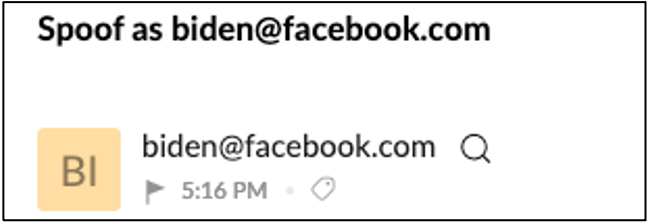
\includegraphics[width=\columnwidth]{graphs/ss_zoho_arc.png}}
%   \centering
%   \caption{An email spoofing \dns{biden@facebook.com} via Fastmail.}
%   \label{fig:ss_zoho_arc}
%   \end{figure}

%Figure~\ref{fig:ss_zoho_arc} in the Appendix illustrates that this attack succeeds without any security warnings, even though the spoofed domain in our
%experiment, \dns{facebook.com}, has a DMARC policy of \textsc{Reject}.



% \subsubsection*{Impact and Mitigation}
% Among providers that I studied, this attack affects customers with
% Zoho email addresses or using Zoho email services,\footnote{We
%   speculate that the above attack also works for customers using Zoho
%   email services, but I are not able to verify this because I are
%   not a Zoho customer.} which together compromise more than 10 million
% potential victims~\cite{Celebrat69:online}.

% However, the attack depends on the existence of providers that allow
% open forwarding and that the receiving provider misinterprets ARC
% headers.  Eliminating either of these factors would foreclose the attack.


\subsection{Abusing Mailing Lists}
\label{subsec:attack_none_mailing_list}

% \subsubsection*{Attack Overview}
The final attack allows an adversary to abuse the forwarding process
used by mailing lists so that spoofed email, which would otherwise
fail DMARC authentication checks, successfully passes both SPF and
DMARC validation.
This attack targets domains with a weak DMARC policy of \textsc{None},
and exploits the way in which many mailing lists rewrite email headers during their forwarding process.
Concretely, this attack allows an adversary to abuse REM header rewriting (\S~\ref{sec:measure_forwarding_mechs_and_arc}) to launder spoofed email through mailing lists such that the forwarded email appears as if it originated from the legitimate sender, even though the original email fails DMARC authentication.\footnote{One such attack used to distribute phishing messages at our institution was part of the impetus for this study.}

% successfully spoof email from any address within an
% organization that uses a vulnerable mailing list service;
% the header rewriting performed by mailing lists makes the spoofed email appear as if originated from the legitimate sender.
% As a result, the attack takes advantage of the header rewriting
% performed by mailing lists to have the spoofed email's headers appear
% as if it originated from the legitimate sender.
%% \geoff{does Sec 4
%%   discuss why mailing lists are designed to work this way, e.g., why
%%   it might have been reasonable for them to work this way?}\alex{Will
%%   add the movitation behind how mailing list operates in sec 2/3,
%%   revisit this later.}

% \subsubsection*{Impact}
%\paragraph{Impact}
\paragraph{Scope}
Our experiments show that attackers can
conduct this attack across all four popular mailing list services: Google
Groups, Mailman, Listserv, and Gaggle.

This attack only affects organizations that use a mailing list configured under their own domain name, and with a DMARC policy of \textsc{None} for their (sub)domain.
While these requirements appear restrictive, prior
work has found that many organizations
(such as major U.S.\ universities) have exactly this configuration~\cite{hutowardsunderstanding}.
Indeed, in querying \dns{.edu} and
\dns{.gov} domains, roughly 10\% of all \dns{.edu}
domains and 5\% of all \dns{.gov} domains are potentially susceptible to this attack.\footnote{As examples, Yale University operates \dnsfn{yale.edu} with a DMARC policy of \textsc{None} and hosts multiple mailing lists using Mailman, and the State of Washington operates a range of mailing lists using Listserv and whose \dnsfn{wa.gov} domain also has a DMARC policy of \textsc{None}.}




% \subsubsection*{Threat Model and Attack Procedure}
%\paragraph{Attack Procedure}
\paragraph{Example}
%In this attack, adversaries control a malicious server that can send spoofed email messages and aim to spoof email from a domain that hosts a mailing list with REM forwarding (Section~\ref{sec:background:fwdingflow}),
%such as Google Groups, Mailman, and Listserv.
%For this attack to work, the spoofed domain must have a DMARC policy of None,
%and the sending email address the attacker wishes to impersonate must have permission to send to the mailing list.
% This attack assumes that only the sender is malicious --- that the adversary controls a server capable of sending spoofed email messages. Additionally, I assume that the domain the adversary wishes to spoof (\dns{univ.edu}) hosts a mailing list with one of these providers,
% such as \dns{list@univ.edu} if they use Google Groups, or \dns{list@listserv.univ.edu} if they use Listserv.
% For this attack to work, \dns{univ.edu} must have a DMARC policy of none,
% and the \dns{univ.edu} email address the attacker wishes to impersonate must have permission to send to the mailing list.
Figure~\ref{fig:google_groups_mech} describes an example of this attack
using Google Groups.
First, an attacker selects a target email address (\dns{someone@univ.edu}) to impersonate in their spoofed email,
and sends the spoofed message from their malicious server to the organization's mailing list (\dns{list@univ.edu}).
Although the email fails DMARC validation,
the mailing list will still accept the message (because \dns{univ.edu}
has a DMARC policy of \textsc{None}).
As part of REM forwarding, the mailing list will rewrite the
\textsc{MAIL FROM} header such that its domain matches the mailing
list's domain, and then forward the email to the list's members.
%(\eg, a new \textsc{MAILFROM} address of
%\dns{xyz@univ.edu}).\footnote{The exact username (the ``xyz'' part) in
%  the \textsc{MAILFROM} address after rewriting depends on the
%  specific implementation.}
As a result, when a recipient's server receives the message it will
successfully pass SPF validation since the domain of the rewritten
\textsc{MAIL FROM} (\dns{univ.edu}) allows the mailing list to send on
its behalf.
Moreover, the spoofed message will also pass DMARC alignment checks,
since the rewriting performed during REM forwarding
ensures that the \textsc{MAIL FROM} and \textsc{FROM} domains are
identical.\footnote{Note that while our examples show this attack
using the organization's top-level domain, it is also effective for
any of the organization's subdomains (if the subdomains also have
DMARC policy \textsc{None}) due to DMARC's inherent relaxed alignment policy.}

During our experiments, I also observed that some mailing list
services, such as Gaggle, do not enforce DMARC policies at all.
This lack of enforcement allows the attack to succeed regardless of the spoofed domain's DMARC policy.




